\documentclass[twoside,11pt]{homework}

\coursename{COMS 4771 Machine Learning 2020} 

\studname{Joseph High \& Eliza Mace}    % YOUR NAME GOES HERE
\studmail{jph2185,emm2314}% YOUR UNI GOES HERE
\hwNo{1}                   % THE HOMEWORK NUMBER GOES HERE
\date{\today} % DATE GOES HERE

% Uncomment the next line if you want to use \includegraphics.
\usepackage{graphicx}
%\usepackage{fancyhdr}
\usepackage{enumerate}
\usepackage{amsmath}
\usepackage{relsize}
\usepackage{mathtools}
\usepackage[dvipsnames]{xcolor}
\usepackage{collectbox}
\usepackage{cancel}

\makeatletter
\newcommand{\mybox}{%
    \collectbox{%
        \setlength{\fboxsep}{1pt}%
        \fbox{\BOXCONTENT}%
    }%
}

\DeclarePairedDelimiter{\2norm}{\lVert}{\rVert^2_2}
\newcommand{\defeq}{\vcentcolon=}
\newcommand\unif{\ensuremath{\operatorname{unif}}}

%%%%%%% %%%%%%%%% Direct Comments %%%%%%%%%%%%%
\newcommand{\joe}[1]{\textcolor{yellow}{\colorbox{blue}{\parbox{15.5cm}{\textbf{\textsc{Joe}: \ #1}}}}}
%newcommand{\joe}[1]{}
\newcommand{\eliza}[1]{\textcolor{black}{\colorbox{cyan}{\parbox{15.5cm}{\textbf{\textsc{Eliza}: \ #1}}}}}
%newcommand{\eliza}[1]{}
\newcommand{\zach}[1]{\textcolor{blue}{\colorbox{gray}{\parbox{15.5cm}{\textbf{\textsc{Zach}: \ #1}}}}}
%newcommand{\zach}[1]{}
%%%%%%%%%%%%%%%%%%%%%%%%%%%%%%%%%%%%%%%%

\begin{document}
\maketitle

\section*{Problem 1: Statistical Estimators}
\joe{This is my version of Problem 1. Eliza's is on the following page. Let's revise and possibly combine later.}
\begin{enumerate}[\bf (i)]
\item We are given that $x_1, \dots, x_n$ \ are drawn independently from \\\
$\mathlarger{p \left(x \vert \theta = (a, b) \right) \propto \begin{cases} 1  & \textrm{if } \ a \leq x \leq b  \\   0  & \textrm{otherwise} \end{cases}} \ .$ \\\
\\\
That is,  $x_i  \overset{\rm iid}{\sim} \unif[a, b] \ , \ \forall i \in \{1, \dots, n\}$. Then for each $i$, the pdf of $x_i$ is  \\\
\\\
$\mathlarger{p \left(x_i \vert \theta \right) = \begin{cases} \frac{1}{b-a}  & \textrm{if } \ a \leq x_i \leq b  \\   0  & \textrm{otherwise} \end{cases}}$. \ Therefore, the likelihood function is \\\
\\\
$\mathlarger{\mathcal{L}(\theta | X) = {\displaystyle \prod_{i=1}^{n} p(x_i|\theta)}={\displaystyle \prod_{i=1}^{n} \frac{1}{b-a}=\frac{1}{(b-a)^n}}}$, \ for $\ \ a \leq x_i \leq b \ \ \forall i \in \{1, \dots, n\}$ \\\ 
\\\
The constraints on $\theta$ can be written equivalently as $a \leq \min_i\{x_i\}$ and $b \geq \max_i\{x_i\}$.\\\
\\\
The values of $a$ and $b$ that maximize $\frac{1}{(b-a)^n}$ are equivalent to the values of $a$ and $b$ that minimize $b-a$. Subject to the constraints, $b-a$ is minimized when $a = \min_i\{x_i\}$ and $b = \max_i\{x_i\}$ (both of which are feasible). The MLE estimate of $\theta = (a, b) $, denoted by $\theta_{ML}$, is then
$$\theta_{ML} = \argmax_{\theta}{\mathcal{L}(\theta | X)} = \argmax_{a\leq x_i \leq b}\frac{1}{(b-a)^n} = \argmin_{a\leq x_i \leq b}(b-a) = (\min_i\{x_i\} \ , \ \max_i\{x_i\})$$
Therefore, $$\theta_{ML} = (\min\{x_1, \dots,x_n\} , \ \max\{x_1, \dots, x_n\})$$ 

\item \begin{proof}
For an arbitrary, differentiable function $g$, let $\Gamma$ be such that $g : \Omega \longrightarrow \Gamma$, where $\Omega$ is the parameter space. That is, $\Gamma \defeq \{\tau : g(\theta) = \tau\}$. For each $\tau \in \Gamma$, define $\mathlarger{\Theta_{\tau} \defeq \{\theta : g(\theta) = \tau\}}$, and note that $\Theta_{\tau} \subseteq \Omega$. Finally, let $\hat{\tau}$ be the $MLE$ of $g(\theta)$. That is, $$\hat{\tau} = \argmax_{\tau \in \Gamma}\left(\max_{\theta \in \Theta_{\tau}} \log \mathcal{L}(\theta \vert \textbf{x})\right)$$

%For each $\tau \in \Gamma$, maximize $\log \mathcal{L}(\theta \vert \textbf{x})$ over all values $\theta \in \Theta_{\tau}$, and subsequently maximize over $\tau \in \Gamma$. The result is the maximum over the entire parameter space, $\Omega$, which is equivalent to the maximum likelihood over all $\theta \in \Omega$: 

%$$\mathlarger{\max_{\tau \in \Gamma}\left(\max_{\theta \in \Theta_{\tau}} \log \mathcal{L}(\theta \vert \textbf{x})\right)  = \max_{\theta \in \Omega} \log \mathcal{L}(\theta \vert \textbf{x}) = \log \mathcal{L}(\theta_{ML} \vert \textbf{x})}$$

Since $\Theta_{\tau} \subseteq \Omega$, \ \ $\mathlarger{\max_{\theta \in \Theta_{\tau}}  \log \mathcal{L}(\theta \vert \textbf{x})} \  \leq  \ \mathlarger{\max_{\theta \in \Omega} \log \mathcal{L}(\theta \vert \textbf{x})} = \mathlarger{\log \mathcal{L}(\theta_{ML} \vert \textbf{x})} \ ,$ for all $\tau \in \Gamma$.

That is, since $\log \mathcal{L}(\theta \vert \textbf{x})$ is maximized by $\theta_{ML}$ over all $\theta \in \Omega$, then it also maximizes $\log \mathcal{L}(\theta \vert \textbf{x})$ over $\Theta_{\tau} \subseteq \Omega$, for all $\tau \in \Gamma$. More specifically, 
%In particular, for some $\theta_{0} \in \mathlarger{\mathlarger{\Theta_{\hat{\tau}}}} = \{\theta : g(\theta) = \hat{\tau}\} \ $ (i.e., $g(\theta_0) = \hat{\tau}$), we have that $\log \mathcal{L}(\theta_0 \vert \textbf{x}) \leq \log \mathcal{L}(\theta_{ML} \vert \textbf{x})$.

$$\mathlarger{\max_{\tau \in \Gamma}\left(\max_{\theta \in \Theta_{\tau}} \log \mathcal{L}(\theta \vert \textbf{x})\right)  = \max_{\theta \in \Omega} \log \mathcal{L}(\theta \vert \textbf{x}) = \log \mathcal{L}(\theta_{ML} \vert \textbf{x})}$$

Then it must be the case that $\theta_{ML} \in \mathlarger{\mathlarger{\Theta_{\hat{\tau}}}} = \{\theta : g(\theta) = \hat{\tau}\}$

$ \Longrightarrow \  g(\theta_{ML}) = \hat{\tau}$. Hence, $g(\theta_{ML})$ is the MLE of $g(\theta)$.

\end{proof}

\item  
\begin{itemize}
\item \textit{Consistent and unbiased}:  (i) $\hat{\mu} = \mathlarger{\frac{1}{N}\sum_{i=1}^N X_i}$ and (ii) a linear combination of the data with unequal weights on each data point: 

 $\hat{\mu} = \mathlarger{\sum_{i=1}^N \gamma_i X_i} \textrm{ where } \gamma_i \neq \gamma_j \textrm{ and } \sum_{i = 1}^N \gamma_i = 1$

For each estimator, we will show why each estimate is consistent and unbiased.\\*

(i) \mybox{$\hat{\mu} = \mathlarger{\frac{1}{N}\sum_{i=1}^N X_i}$} 

\underline{Unbiased}: \  $\mathbb{E}[\hat{\mu}] = \mathbb{E}\left[\mathlarger{\frac{1}{N}\sum_{i=1}^N X_i}\right] = \mathlarger{\frac{1}{N}
\sum_{i=1}^N \mathbb{E}[X_i]} = \mathlarger{\frac{1}{N}\sum_{i=1}^N \mu} = \mu$ \\*
\\\

\underline{Consistent}: \ $$\lim_{N \to \infty} \mathbb{E}[\hat{\mu}] = \lim_{N \to \infty}\mathbb{E}\left[\frac{1}{N}\sum_{i=1}^N X_i\right] = \lim_{N \to \infty}\frac{1}{N}\sum_{i=1}^N \mu = \lim_{N \to \infty}\mu = \mu$$
and 
\begin{multline*}
\lim_{N \to \infty} \text{Var} [\hat{\mu}] = \lim_{N \to \infty} \text{Var} \left[\frac{1}{N}\sum_{i=1}^N X_i \right] = \lim_{N \to \infty} \frac{1}{N^2}\sum_{i=1}^N \text{Var} [X_i] = \lim_{N \to \infty} \frac{N\sigma^2}{N^2} = \lim_{N \to \infty} \frac{\sigma^2}{N} = 0
\end{multline*}

(ii) \mybox{$\mathlarger{\hat{\mu}= \mathbb{E}\left[\sum_{i=1}^N \gamma_i X_i\right] } \textrm{ where } \gamma_i \neq \gamma_j \textrm{ and } \mathlarger{\sum_{i = 1}^N \gamma_i = 1}$}

\underline{Unbiased}: \ $$\mathbb{E}[\hat{\mu}] = \mathbb{E}\left[\sum_{i=1}^N \gamma_i X_i\right] =
\sum_{i=1}^N \gamma_i \mathbb{E}[X_i] = \sum_{i=1}^N \gamma_i \mu = \mu\sum_{i=1}^N \gamma_i = \mu \times 1 = \mu$$


\underline{Consistent}: $$\lim_{N \to \infty} \mathbb{E}[\hat{\mu}] = \lim_{N \to \infty}\mathbb{E}\left[\sum_{i=1}^N \gamma_i X_i\right] = \lim_{N \to \infty}\sum_{i=1}^N \gamma_i \mu = \lim_{N \to \infty}\mu = \mu$$
%and 
%\begin{multline*}
%\lim_{N \to \infty} \text{Var} [\hat{\mu}] = \lim_{N \to \infty} \text{Var} \left[\sum_{i=1}^N \gamma_i X_i \right] = \lim_{N \to \infty} \sum_{i=1}^N \gamma_i^2 \text{Var} [X_i] = \lim_{N \to \infty} \frac{N\sigma^2}{N^2} = \lim_{N \to \infty} \frac{\sigma^2}{N} = 0
%\end{multline*}

\item \textit{Consistent, but not unbiased}: (i) $\mathlarger{\hat{\mu} = \frac{1}{N-1}{\displaystyle \sum_{i=1}^{N}X_i}} \ $  \ and (ii) $ \ \mathlarger{\hat{\mu}= \frac{1}{N}{\displaystyle \sum_{i=1}^{N}X_i+\frac{1}{N}}}$

For each estimator, we will show why each estimate is consistent and biased.\\*

(i) \mybox{$\hat{\mu} = \mathlarger{\frac{1}{N-1}\sum_{i=1}^N X_i}$} 

\underline{Biased}: \  $\mathbb{E}[\hat{\mu}] = \mathbb{E}\left[\mathlarger{\frac{1}{N-1}\sum_{i=1}^N X_i}\right] = \mathlarger{\frac{1}{N-1} \sum_{i=1}^N \mathbb{E}[X_i]} = \mathlarger{\frac{1}{N}\sum_{i=1}^N \mu = \frac{N\mu}{N-1}} \neq \mu$


\underline{Consistent}: \  
\begin{multline*}
\lim_{N \to \infty} \mathbb{E}[\hat{\mu}] = \lim_{N \to \infty}\mathbb{E}\left[\frac{1}{N-1}\sum_{i=1}^N X_i\right] = \lim_{N \to \infty}\frac{1}{N-1}\sum_{i=1}^N \mu = \lim_{N \to \infty}\frac{N\mu}{N-1} = \mu  
\end{multline*}
and
\begin{multline*}
\lim_{N \to \infty} \text{Var} [\hat{\mu}] =\lim_{N \to \infty} \text{Var} \left[\frac{1}{N-1}\sum_{i=1}^N X_i\right] \\\ = \lim_{N \to \infty} \left(\frac{1}{N-1}\right)^2 \sum_{i=1}^N \sigma^2  = \lim_{N \to \infty} \frac{N \sigma^2}{(N-1)^2} = \lim_{N \to \infty} \frac{\sigma^2}{N - 2 + \frac{1}{N}} = 0
\end{multline*}


(ii) \mybox{$\mathlarger{\hat{\mu}= \frac{1}{N}{\displaystyle \sum_{i=1}^{N}X_i+\frac{1}{N}}}$} 

\underline{Biased}: \  \begin{multline*} \mathbb{E}[\hat{\mu}] = \mathbb{E}\left[\mathlarger{\frac{1}{N}\sum_{i=1}^N X_i + \frac{1}{N}}\right] = \mathbb{E}\left[\mathlarger{\frac{1}{N}\sum_{i=1}^N X_i}\right] + \mathbb{E}\left[\mathlarger{\frac{1}{N}}\right] = \mathlarger{\frac{1}{N} \sum_{i=1}^N \mathbb{E}[X_i] + \frac{1}{N}} \\ = \mathlarger{\frac{1}{N} \sum_{i=1}^N \mu + \frac{1}{N}} = \mathlarger{\mu + \frac{1}{N}} \neq \mu
\end{multline*}

\underline{Consistent}: \ 
\begin{multline*}
\lim_{N \to \infty} \mathbb{E}[\hat{\mu}] = \lim_{N \to \infty}\mathbb{E}\left[\frac{1}{N}\sum_{i=1}^N X_i + \frac{1}{N}\right] = \lim_{N \to \infty}\left(\frac{1}{N}\sum_{i=1}^N \mu \ + \ \frac{1}{N}\right) = \lim_{N \to \infty}\left(\mu + \frac{1}{N}\right) = \mu
\end{multline*}

\begin{multline*}
\lim_{N \to \infty} \text{Var} [\hat{\mu}] = \lim_{N \to \infty} \text{Var} \left[\frac{1}{N}\sum_{i=1}^N X_i + \frac{1}{N}\right] = \lim_{N \to \infty} \frac{1}{N^2}\sum_{i=1}^N \text{Var} [X_i] = \lim_{N \to \infty} \frac{N\sigma^2}{N^2} \\ = \lim_{N \to \infty} \frac{\sigma^2}{N} = 0
\end{multline*}

\item \textit{Not consistent, but unbiased}: (i) $\hat{\mu} = X_k \in \{X_1, \dots, X_N\}$ \ and \ (ii) $\hat{\mu} = \frac{X_1 + X_2}{2} $

For each estimator, we will show why each estimate is not consistent, but unbiased.\\*

(i) \mybox{$\hat{\mu} = X_k$} 

\underline{Unbiased}: \ $\mathbb{E}[\hat{\mu}] = \mathbb{E}[X_k] = \mu$


\underline{Not consistent}: \ Inconsistent since $X_k$ is fixed and will not change as $N \longrightarrow \infty$. That is,

$$\lim_{N \to \infty} \text{Var} [\hat{\mu}] = \lim_{N \to \infty} \text{Var} [X_k]  = \lim_{N \to \infty} \sigma^2 = \sigma^2 \neq 0 $$


(ii) \mybox{$\hat{\mu} = \frac{X_1 + X_2}{2} $}

\underline{Unbiased}: \ 
$\mathbb{E}[\hat{\mu}] = \mathbb{E}\left[ \frac{X_1 + X_2}{2}\right] = \frac{1}{2}\mathbb{E}[X_1] + \frac{1}{2}\mathbb{E}[X_2] = \frac{1}{2}\mu + \frac{1}{2}\mu
= \mu$


\underline{Not consistent}: \ $$\lim_{N \to \infty} \text{Var} [\hat{\mu}] = \lim_{N \to \infty} \text{Var} \left[ \frac{X_1 + X_2}{2}\right]  = \lim_{N \to \infty}\frac{1}{2}\sigma^2 = \frac{\sigma^2}{2} \neq 0 $$


\item \textit{Neither consistent, nor unbiased}: (i) $X_k + \alpha$ \ and \ (ii) $\alpha X_k$, for some $X_k \in \{X_1, \dots, X_N\}$ and a fixed constant $\alpha > 1$

For each estimator, we will show why each estimate is neither consistent, nor unbiased.\\*

(i) \mybox{$\hat{\mu} = X_k + \alpha$} 

\underline{Biased}: \ $\mathbb{E}[\hat{\mu}] = \mathbb{E}[X_k + \alpha] = \mu + \alpha \neq \mu$


\underline{Not consistent}: \ $$\lim_{N \to \infty} \mathbb{E}[\hat{\mu}] = \lim_{N \to \infty} \mathbb{E}[X_k + \alpha] = \lim_{N \to \infty} \mu + \alpha = \mu + \alpha \neq \mu$$
and
$$\lim_{N \to \infty} \text{Var} [\hat{\mu}] = \lim_{N \to \infty} \text{Var} [X_k + \alpha]  =  \lim_{N \to \infty} \text{Var} [X_k] = \lim_{N \to \infty} \sigma^2 = \sigma^2 > 0$$


(ii) \mybox{$\hat{\mu} = \alpha X_k$}

\underline{Biased}: \ $\mathbb{E}[\hat{\mu}] = \mathbb{E}[\alpha X_k] = \alpha \mu \neq \mu$


\underline{Not consistent}: \ 
$$\lim_{N \to \infty} \mathbb{E}[\hat{\mu}] = \lim_{N \to \infty} \mathbb{E}[\alpha X_k] = \lim_{N \to \infty} \alpha \mu = \alpha \mu \neq \mu$$
and 
$$\lim_{N \to \infty} \text{Var} [\hat{\mu}] = \lim_{N \to \infty} \text{Var} [\alpha X_k]  = \lim_{N \to \infty}\alpha^2 \sigma^2 = \alpha^2 \sigma^2 > 0$$

\end{itemize}
\end{enumerate}


%\section*{Problem 1: Statistical Estimators}
%\begin{enumerate}[(i)]
%	\item
%	\begin{equation*}
%	P(X|\theta=(a,b))\propto
%	\begin{cases}
%	1 & a \leq x \leq b \\
%	0 &\text{otherwise}
%	\end{cases}
%	\end{equation*}
%	$\mathcal{L}(\theta)={\displaystyle \prod_{i=1}^{N} p(x_i|\theta)}={\displaystyle \prod_{i=1}^{N} \frac{1}{b-a}=\frac{1}{(b-a)^N}}$ \\[10pt]
%	$a\leq min(x_1,...,x_N)$ and $b\geq max(x_1,...,x_N)$ \\[10pt]
%	maximum likelihood ($\mathcal{L}$) is when $b-a$ is as small as possible, so $b=max(x_i)$ and $a=min(x_i)$\\[10pt]
%	$MLE(\theta)=(min(x_i),max(x_i))$	
%	\item Invariance property of MLE's \\
%	if $g$ is one-to-one:\\
%	$\mathcal{L}(\theta) = \mathcal{L}(g^(-1)(g(\theta)))$\\[10pt]
%	Likelihood is maximized by $\theta_{ML}$:\\
%	$\theta_{ML}=g^{-1}(ML(g(\theta)))$ \\[10pt]
%	$g(\theta_{ML})=ML(g(\theta))$\\[10pt]
%	if $g$ is many-to-one:\\
%	HELP!
%	\item For 1-dim Gaussian
%	\begin{itemize}
%		\item consistent and unbiased:
%		$\mu = \frac{1}{N}{\displaystyle \sum_{i=1}^{N}x_i}$
%		\item consistent, but not unbiased:
%		$\mu = \frac{1}{N-1}{\displaystyle \sum_{i=1}^{N}x_i}$ and $\mu = \frac{1}{N}{\displaystyle \sum_{i=1}^{N}x_i+\frac{1}{N}}$
%		\item not consistent, but unbiased:
%		\item neither consistent, nor unbiased:
%		$\mu = constant \neq \hat{\mu}$
%	\end{itemize}
%\end{enumerate}

\section*{Problem 2: On Forecasting Product Demand}
\begin{enumerate}
	\item 
	\begin{equation*}
	\begin{split}
	\pi(D) &= \int_{0}^{Q-1}[(P-C)\cdot D-C\cdot (Q-D)]\cdot f(D)dD+\int_{Q}^{\infty}(P-C)\cdot Q\cdot f(D)dD\\
	&= \int_{0}^{Q-1}[(P-C)D-C(Q-D)]\cdot f(D)dD+(P-C)\cdot Q[ 1-\int_{0}^{Q-1}f(D)dD]\\
	&=\int_{0}^{Q-1}P\cdot D\cdot f(D)dD-C\cdot Q\int_{0}^{Q-1}f(D)dD+(P-C)\cdot Q+(P-C)\cdot Q \int_{0}^{Q-1}f(D)dD\\
	&=(P-C)\cdot Q+P\int_{0}^{Q-1}D\cdot f(D) dD + [(P-C)\cdot Q-C\cdot Q]\int_{0}^{Q-1}f(D)dD\\
	&=(P-C)\cdot Q+P\int_{0}^{Q-1}D\cdot f(D)dD+[Q\cdot(P-2C)][F(Q-1)-F(0)]
	\end{split}
	\end{equation*}
	\item 
	\begin{equation*}
	\begin{split}
	\frac{d\pi}{dQ}&=(P-C)+P\cdot(Q-1)\cdot f(Q-1)+\frac{d}{dQ}[(P-2C)\cdot Q\cdot F(Q-1)-(P-2C)\cdot Q \cdot F(0)]\\
	\end{split}
	\end{equation*}
\end{enumerate}

\section*{Problem 3: Evaluating Classifiers}
\begin{enumerate}[(i)]
	\item We get an error when $x_i>t,y_i=y_2$ or when $x_i\leq t,y_i=y_1$\\
	\begin{equation*}
	\begin{split}
	P[f_t(X)\neq y]&=P[f_t(\vec{x})=y_1,Y=y_2|X=\vec{x}]+P[f_t(\vec{x})=y_2,Y=y_1|X=\vec{x}]\\
	&=P[x_i>t,Y=y_2|X=x_i]+P[x_i\leq t,Y=y_1|X=x_i]
	\end{split}
	\end{equation*}
	$f_t(x)$ is conditionally independent of $y$ given $x$
	\begin{equation*}
	\begin{split}
	P[f_t(x)\neq y]&=P[x_i>t|X=x_i]P[Y=y_2|X=x_i]+P[x_i\leq t|X=x_i]P[Y=y_1|X=x_i]\\
	&=\mathbb{1}(x_i>t)P[Y=y_2,X=x_i]+(1-\mathbb{1}(x_i>t))P[Y=y_i|X=x_i]
	\end{split}
	\end{equation*}
	\item optimal threshold
	\item bayes error rate
\end{enumerate}

\section*{Problem 4: Analyzing iterative optimization}
\begin{enumerate}[\bf (i)]
	% Prove M is symmetric PSD
	\item 
	\begin{proof}
	%Symmetric
	 We first show that $M$ is \textit{symmetric}. \\ Recall that a (square) matrix $M$ is symmetric $\Longleftrightarrow M = M^{\top}$   \\
	 Clearly, $M = A^{\top}A$ is a square matrix ($A^{\top}A$ a $d \times d$ matrix). Consider the following $$M^{\top} = (A^{\top}A)^{\top} = A^{\top}(A^{\top})^{\top} = A^{\top}A = M
	\Longrightarrow \ M^{\top} = M$$ Thus, $M$ is symmetric. 
	
	%Positive semi-definite
	To prove that $M$ is also \textit{positive semi-definite}, it suffices to show that for any \\ $x \in \mathbb{R}^d, \ x^{\top}Mx \geq 0$. As such, consider an arbitrary vector $\textbf{x} \in \mathbb{R}^d$ and let $\textbf{w} = A\textbf{x}$, where $\textbf{w} \in \mathbb{R}^n$ and $\textbf{w} = [w_1, \ w_2, \ \dots, w_n]^{\top}$. We then have that, 
	$$\textbf{x}^{\top}M\textbf{x} = \textbf{x}^{\top}A^{\top}A\textbf{x} = (A\textbf{x})^{\top}A\textbf{x} = \2norm{A\textbf{x}} = \2norm{\textbf{w}} = \sum^n_{i = 1}w^2_i  \geq 0$$
	$\Longrightarrow M$ is positive semi-definite. 
\end{proof}	

    % Prove equivalent form of iteration by induction
	\item \begin{proof} Proof by induction on $N$.
	
	\underline{Base case} ($N = 1, 2$) 
	
	For $N = 1$ we have
	\vspace{-0.05in}
	\begin{align*} 
	\beta^{(1)} & = \beta^{(0)} + \eta A^{\top}(b - A\beta^{(0)}) && \text{(by definition of the Richardson iteration)}\\
	& =  \eta A^{\top}b = \eta v && \text{(since $\beta^{(0)}$ is the zero vector and $v = A^{\top}b$)} \\	
	& =  \eta I v = \eta \underbrace{(I - \eta M)^0}_{= I}v && \text{(Note: $(I-\eta M)$ is a square matrix since $I$ and $M$ are square)} \\
	& = \eta \sum_{k=0}^0 (I - \eta M)^kv && \text{Thus, it holds for $N = 1$.}
    \end{align*}
    
    For $N = 2$ we have
    \vspace{-0.05in}
	\begin{align*}
	\beta^{(2)} & = \beta^{(1)} + \eta A^{\top}(b - A\beta^{(1)}) =  \eta v + \eta (A^{\top}b - A^{\top}A\eta v) && \text{(since $\beta^{(1)} = \eta v$ from the above)}\\
	& = \eta v + \eta (v - M\eta v) && \text{(since $M = A^{\top}A$ and $v = A^{\top}b$)}\\
	& = \eta \underbrace{(I - \eta M)^0}_{= I} v + \eta(I - \eta M)v && \text{($\eta$ a real number)}\\
	& = \eta[(I - \eta M)^0 v + (I - \eta M)^1v] \\
	& = \eta \sum_{k=0}^{1} (I - \eta M)^kv && \text{Thus, it holds for $N=2$.}
     \end{align*}
	
	(Inductive hypothesis) Now assume the result holds for $k = 1, 2, \dots, N-1$. \\* That is, assume the following holds:
	$$\beta^{(N-1)} = \eta \sum_{k=0}^{N-2} (I - \eta M)^kv$$
	From the definition of the Richardson iteration, the $N^{th}$ iterate is
	\begin{align*}
	\beta^{(N)} & = \beta^{(N-1)} + \eta A^{\top}(b - A\beta^{(N-1)}) = \beta^{(N-1)} + \eta (v- M\beta^{(N-1)}) \\
	& = \eta \sum_{k=0}^{N-2} (I - \eta M)^kv + \eta \left[v - M\left(\eta \sum_{k=0}^{N-2} (I - \eta M)^kv\right)\right] && \text{(from the induction hypothesis)}\\
	& = \eta \sum_{k=0}^{N-2} (I - \eta M)^kv - \eta M\left(\eta \sum_{k=0}^{N-2} (I - \eta M)^kv\right) + \eta v \\
	& = (I - \eta M)\left(\eta \sum_{k=0}^{N-2} (I - \eta M)^kv\right) + \eta v \\
	& = \eta \sum_{k=0}^{N-2} (I - \eta M)^{k+1}v + \eta v \\
	& = \eta \sum_{k=1}^{N-1} (I - \eta M)^{k}v + \eta v && \text{(rearrange indices)}\\
	& = \eta \sum_{k=1}^{N-1} (I - \eta M)^{k}v + \eta \underbrace{(I - \eta M)^0}_{= I} v && \text{(adding $k = 0$ summand)}\\
	& = \eta \sum_{k=0}^{N-1} (I - \eta M)^{k}v 
	\end{align*}
	Hence, \ $\mathlarger{\beta^{(N)} = \eta \sum_{k=0}^{N-1} (I - \eta M)^{k}v}$
	\end{proof}
	
	% eigenvalues
	\item We are given that the eigenvalues of $M$ are $\lambda_1, \lambda_2, \dots, \lambda_d$. Then, the eigenvalues of $I - \eta M$ are $1-\eta \lambda_i$, for all $i = 1, \dots, d$. Indeed, without loss of generality, let $\textbf{x}$ be the eigenvector associated with $\lambda_i$, then $M\textbf{x} = \lambda_i\textbf{x} \  \Longrightarrow \ (\eta M)\textbf{x} = (\eta \lambda_i)\textbf{x} \  \Longrightarrow \ I\textbf{x} - (\eta M)\textbf{x} = I\textbf{x} - \eta \lambda_i\textbf{x} = 1\textbf{x} - \eta \lambda_i\textbf{x} \ \Longrightarrow \ (I - \eta M)\textbf{x} = (1 - \eta \lambda_i)\textbf{x}$. 
	
%By a similar argument, we can also conclude that the eigenvalues of $\eta(I - \eta M)$ are $\eta(1-\eta\lambda_i)$.
	
	We also claim that since $((1-\eta\lambda_i), \ \textbf{x})$ is the eigenvalue--eigenvector pair for $(I - \eta M)$, then $((1-\eta\lambda_i)^k, \ \textbf{x})$ is the eigenvalue--eigenvector pair for $(I - \eta M)^k \ , \ k \in \mathbb{N}\cup \{0\}$. 
	
	\textit{Proof of claim}: For any $i \in \{1, 2, \dots, d\}$ we have
	 \begin{align*} 
	(I - \eta M)\textbf{x} = (1 - \eta \lambda_i)\textbf{x} \ & \Longrightarrow \ (I - \eta M)^2\textbf{x} = (1 - \eta \lambda_i)(I - \eta M)\textbf{x} = (1 - \eta\lambda_i)^2\textbf{x} \\
& \Longrightarrow \ (I - \eta M)^3\textbf{x} = (1 - \eta \lambda_i)^2(I - \eta M)\textbf{x} = (1 - \eta\lambda_i)^3\textbf{x} \\
 & \vdots \\
 & \Longrightarrow \ (I - \eta M)^k\textbf{x} = (1 - \eta \lambda_i)^{k-1}(I - \eta M)\textbf{x} = (1 - \eta\lambda_i)^k\textbf{x}\\
 && \square
	\end{align*}
%For a polynomial $p(t) = \alpha_0 + \alpha_1 t + \alpha_2 t^2 + \dots + \alpha_n t^n$ and some square matrix $A$, define $p(A)$ to be the matrix $p(A) = \alpha_0 I + \alpha_1 A + \alpha_2 A^2 + \dots + \alpha_n A^n = \sum_{k=0}^n \alpha_k A^k$, where  $\alpha_i = \eta$ for all $i = 1, \dots, n$. We claim that the eigenvalue--eigenvector pair for $p(I - \eta M)$ is  $((1-\eta \lambda_i), \ \textbf{x})$. 

Using the above results, we have the following
\begin{multline*}
 \eta I\textbf{x} + \eta(I - \eta M)\textbf{x} + \eta(I - \eta M)^2\textbf{x}  + \dots + \eta(I - \eta M)^{N-1}\textbf{x} = \\ \eta \textbf{x} + \eta(1 - \eta \lambda_i)\textbf{x} + \eta(1 - \eta \lambda_i)^2\textbf{x} + \dots + \eta(1 - \eta \lambda_i)^{N-1}\textbf{x} 
\end{multline*}
\vspace{-0.3in}
\begin{multline*}
 \Longrightarrow \eta(I + (I - \eta M) + (I - \eta M)^2  + \dots + (I - \eta M)^{N-1})\textbf{x} = \\ \eta(1 + (1 - \eta \lambda_i) + (1 - \eta \lambda_i)^2 + \dots + (1 - \eta \lambda_i)^{N-1})\textbf{x} 
\end{multline*}

$\Longrightarrow \mathlarger{\left(\eta \sum_{k = 0}^{N-1}(I - \eta M)^k\right)\textbf{x} = \left(\eta \sum_{k = 0}^{N-1}(1 - \eta \lambda_i)^k\right)\textbf{x}} = \mathlarger{\left(\frac{1 - (1-\eta \lambda_i)^N}{\lambda_i}\right)\textbf{x}}$\ , \ $\forall i = 1, 2, \dots, d$ \\*
\\
Thus, the eigenvalues of $\mathlarger{\eta \sum_{k = 0}^{N-1}(I - \eta M)^k}$ are \ $$\frac{1 - (1-\eta \lambda_1)^N}{\lambda_1} \ , \ \frac{1 - (1-\eta \lambda_2)^N}{\lambda_2} \ , \ \dots \ , \ \frac{1 - (1-\eta \lambda_d)^N}{\lambda_d}$$. 

	%convergence
	\item 
	\begin{proof} 
	\text{} \\
	Note that 
	\begin{align*} 
	 \hat{\beta} - \beta^{(N)} & = \left(\hat{\beta} + \eta A^{\top}(b - A \hat{\beta})\right) - \left(\beta^{(N-1)} + \eta A^{\top}(b - A \beta^{(N-1)})\right) \\ 
	& = \left(\hat{\beta} + \eta v - \eta M \hat{\beta}\right) - \left(\beta^{(N-1)} + \eta v - \eta M \beta^{(N-1)}\right) \\
	& =  \left((I - \eta M)\hat{\beta} + \cancel{\eta v}\right) - \left((I - \eta M)\beta^{(N-1)} + \cancel{\eta v}\right)\\	
	& = (I - \eta M)(\hat{\beta} - \beta^{(N-1)}) \\ 
	& = (I - \eta M)^2((\hat{\beta} - \beta^{(N-2)}) \\
	& = (I - \eta M)^3(\hat{\beta} - \beta^{(N-3)}) \\
	& \vdots \\
	& = (I - \eta M)^N(\hat{\beta} - \beta^{(0)}) \\
	& = (I - \eta M)^N\hat{\beta} \\
	\end{align*}
	
Now consider,
\begin{align*}
\2norm{ \beta^{(N)} - \hat{\beta}} = \2norm{\hat{\beta} - \beta^{(N)}} & = \2norm{(I - \eta M)^N\hat{\beta}} \\ & \leq \2norm{(I - \eta M)^N}\2norm{\hat{\beta}} \\
& \leq (\2norm{(I - \eta M)})^N \2norm{\hat{\beta}} \\
& = \lVert I - \eta M \rVert^{2N}_2 \2norm{\hat{\beta}} \\
& \leq (1 - 2\eta \lambda_{min})^N \2norm{\hat{\beta}} \\
& \leq e^{-2\eta \lambda_{min}N} \2norm{\hat{\beta}}
\end{align*}
	\end{proof}
\end{enumerate}

\section*{Problem 5: Designing socially aware classifiers}

\begin{enumerate}[(i)]
	\item It is not enough just to remove the sensitive attribute \emph{A} from the dataset because it is possible that other attributes in the feature vector are correlated with this attribute.
	\item Demographic parity
	\item equivalence relationship
	\item classifiers
	\item 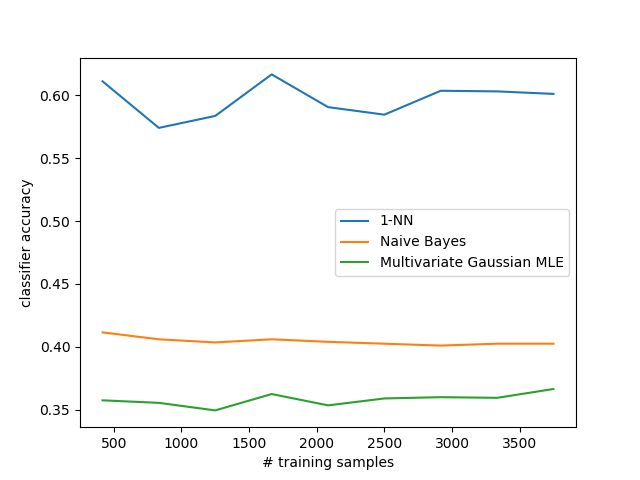
\includegraphics[width=\textwidth]{compas.png}
	\item positive rate across sensitive attribute
	\item real-world
\end{enumerate}

\section*{Problem 6: Email spam classification case study}

\begin{enumerate}[(i)]
	\item Bag-of-words
	\item classifiers
	\item Naive bayes is best!
\end{enumerate}

\end{document} 
